\documentclass[12pt]{jreport}
\usepackage{styles/epsf}
\usepackage{fleqn}
\usepackage{hhline}
\usepackage{styles/soturon}
\usepackage{fancyhdr}
\usepackage[dvipdfm]{graphicx}

\title{ファラデーの電荷研究の実用化に向けて}
\author{大沼 奏太}

\newcommand{\Vec}[1]{{\mbox{\boldmath $#1$}}}
\newcommand{\dfrac}[2]{{\displaystyle \frac{#1}{#2}}}

\newcommand{\figref}[1]{図~\ref{#1}}
\newcommand{\eqref}[1]{式(\ref{#1})}
\newcommand{\tabref}[1]{表~\ref{#1}}
\newcommand{\bibref}[1]{文献~\cite{#1}}

\newcommand{\chref}[1]{第~\ref{#1}~章}
\newcommand{\secref}[1]{第~\ref{#1}~節}

\renewcommand{\thechapter}{\arabic{chapter}}
\renewcommand{\thesection}{\arabic{chapter}.\arabic{section}}
\renewcommand{\thefigure}{\arabic{chapter}.\arabic{figure}}
\renewcommand{\theequation}{\arabic{chapter}.\arabic{equation}}
\renewcommand{\thetable}{\arabic{chapter}.\arabic{table}}

%%%%%%%%%%%%%%%%%%%%%%%%%%%%%
%↑これがあると目次が出ません．
%マニュアルなど参考資料を添付したいときは，参考資料の内容をinputせずに
%目次を作ってから\nofilesで目次を更新しないようにして参考資料をinputします．
%そうすると参考資料はタイトルだけが表示されます．
%%%%%%%%%%%%%%%%%%%%%%%%%%%%%
\begin{document}

\maketitle
\pagenumbering{roman}

\newpage
\chapter*{論文要旨}
\addcontentsline{toc}{chapter}{論文要旨}

偉人の伝記というと，ナポレオンとかアレキサンドロスとか，グラッドストーンというようなのばかりで，学者のはほとんど無いと言ってよい．
なるほどナポレオンやアレキサンドロスのは，雄であり，壮である．
しかし，いつの世にでもナポレオンが出たり，アレキサンドロスの出ずることは出来ない．
文化の進まざる時代の物語りとして読むには適していても，修養の料にはならない．
グラッドストーンのごときといえども，一国について見れば二，三人あり得るのみで，しかも大宰相たるは一時に一人のみしか存在を許さない．
これに反して，科学者や哲学者や芸術家や宗教家は，一時代に十人でも二十人でも存在するを得，また多く存在するほど文化は進む．
ことに科学においては，言葉を用うること少なきため，他に比して著しく世界的に共通で，日本での発見はそのまま世界の発見であり，詩や歌のごとく，外国語に訳するの要もない．

これらの理由により，科学者たらんとする者のために，大科学者の伝記があって欲しい．
しかし，科学者の伝記を書くということは，随分むずかしい．というのは，まず科学そのものを味った人であることが必要であると同時に多少文才のあることを要する．
悲しいかな，著者は自ら顧みて，決してこの二つの条件を備えておるとは思わない．
ただ最初の試みをするのみである．
　
科学者の中で，特にファラデーを選んだ理由は，第一に彼は大学教育を受けなかった人で，全くの丁稚小僧から成り上ったのだ．
学界にでは家柄とか情実とかいうものの力によることがない，腕一本でやれるということが明かになると思う．また立身伝ともいえる．
次に彼の製本した本も，筆記した手帳も，実験室での日記も，発見の時に用いた機械も，それから少し変ってはいるが，実験室も今日そのまま残っている．
シェーキスピアやカーライルの家は残っている．
ゲーテ，シルレルの家もあり，死んだ床も，薬を飲んだ杯までもある（真偽は知らないが）．ファラデーのも，これに比較できる位のものはある．
科学者でファラデーほど遺物のあるのは，他に無いと言ってよい．
それゆえ，伝記を書くにも精密に書ける．
諸君がロンドンに行かるる機会があったら，これらの遺物を実際に見らるることも出来る．
　
第三に，何にか発見でもすると，その道行きは止めにして，出来上っただけを発表する人が多い．
感服に値いしないことはないが，これでは，後学者が発見に至るまでの着想や推理や実験の順序方法について，貴ぶべき示唆を受けることは出来ない．
あたかも雲に聳（そび）ゆる高塔を仰いで，その偉観に感激せずにはいられないとしても，さて，どういう足場を組んで，そんな高いものを建て得たかが，判らないのと同じである．

ファラデーの論文には，いかに考え，いかに実験して，それでは結果が出なくて，しまいにかくやって発見した，というのが，偽らずに全部書いてある．これでこそ発見の手本にもなる．
またファラデーの伝記は決して無味乾燥ではない．電磁気廻転を発見して，踊り喜び，義弟をつれて曲馬見物に行き，入口の所でこみ合って喧嘩をやりかけた壮年の元気は中々さかんである．
莫大の内職をすて，［＃「莫大の内職をすて，」は底本では「莫大の内職をすて，」］宴会はもとより学会にも出ないで，専心研究に従事した時代は感嘆するの外はない，晩年に感覚も鈍り，ぼんやりと椅子（いす）にかかりて，西向きの室から外を眺めつつ日を暮らし，終に眠るがごとくにこの世を去り，静かに墓地に葬られた頃になると，落涙を禁じ得ない．

前編に大体の伝記を述べて，後編に研究の梗概（こうがい）を叙することにした．


\newpage

\tableofcontents
\newpage
\listoffigures
\newpage
\listoftables
\newpage

\pagestyle{fancy}
\rhead{\leftmark}
\lhead{}
\cfoot{\thepage}
\renewcommand{\chaptermark}[1]{\markboth{第\ \thechapter\ 章~#1}{}}

\pagenumbering{arabic}

% 本文
\chapter{序論} \label{chap:jyoron}


\section{研究背景}%\label{sec:background}

前世紀の初めにロンドンのマンチエスター・スクエーアで，走り廻ったり，球をころがして遊んだり，おりおり妹に気をつけたりしていた子供があった．すぐ側のヤコブス・ウエルス・ミュースに住んでいて，学校通いをしていた子供なのだ．
通りがかりの人で，この児に気づいた者は無論たくさんあったであろうが，しかし誰れ一人として，この児が成人してから，世界を驚すような大科学者になろうと思った者があろうか．

この児の生れたのは今いうたミュースではない．只今では大ロンドン市の一部となっているが，その頃はまだロンドンの片田舎に過ぎなかったニューイングトン・ブットが，始じめて呱々（ここ）の声をあげた所で，それは一七九一年九月二十二日のことであった．
父はジェームス・ファラデーといい，母はマーガレットと呼び，その第三番目の子で，ミケルという世間には余り多くない名前であった．
父のジェームスは鍛冶職人（かじしょくにん）で，身体も弱く，貧乏であったので，子供達には早くからそれぞれ自活の道を立てさせた\cite{Furui}．


\section{本研究の目的}%\label{sec:purpose}

\begin{figure}[t]
\begin{center}
\begin{verbatim}
いたっ+イタッ+いたる+44/17/8	[いたっ+イタッ+いたる+44/17/8]	i t a q 
いたって+イタッテ+52	[いたって+イタッテ+52]	i t a q t e 
いたみ+イタミ+いたむ+44/16/6	[いたみ+イタミ+いたむ+44/16/6]	i t a m i 
いため+イタメ+2	[いため+イタメ+2]	i t a m e 
いため+イタメ+いためる+44/6/5	[いため+イタメ+いためる+44/6/5]	i t a m e 
いためる+イタメル+44/6/2	[いためる+イタメル+44/6/2]	i t a m e r u 
いたら+イタラ+いたる+44/17/3	[いたら+イタラ+いたる+44/17/3]	i t a r a 
いたり+イタリ+いたる+44/17/7	[いたり+イタリ+いたる+44/17/7]	i t a r i 
いたる+イタル+44/17/2	[いたる+イタル+44/17/2]	i t a r u 
\end{verbatim}
\caption{単語辞書ファイルの例}
\label{fig:dic}
\end{center}
\end{figure}

前述したようにこんな形で図形とすることもできる．
図~\ref{fig:dic}はほんとうは図ではない．
しかし，次はepsの図を貼り付ける方法である．図~\ref{fig:bigrecgsys}はepsで用意した物だ．

\begin{figure}[t]
\begin{center}
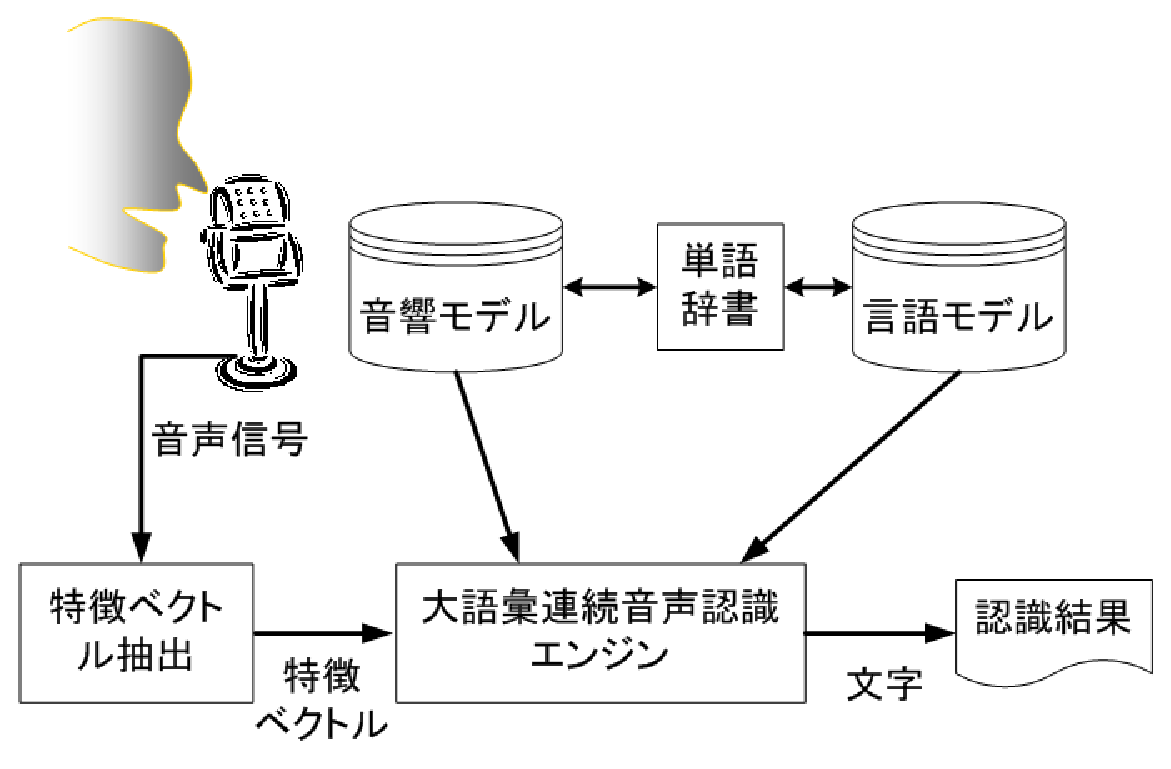
\includegraphics[width=14cm]{figures/recgsys.eps}
\caption{大語彙連続音声認識システム}     
\label{fig:bigrecgsys}
\end{center}
\end{figure}

表も作っておくと，図と表の目次ができる．
表~\ref{table:snr}は表の例である．

\begin{table}[htbp]
\caption{の度数分布}
\label{table:snr}
\begin{center}
\begin{tabular}{|c|r|r|r|} \hline
音素 & 平均フレーム長 & 分散 & 個数 \\ \hline
i & 6.814762 & 11.83095 & 132268 \\ \hline
u & 5.591616 & 10.67492 & 88505 \\ \hline
e & 7.98301 & 13.52340 & 85818 \\ \hline
o & 7.28116 & 14.32611 & 139195 \\ \hline
a: & 13.35346 & 13.50384 & 2054 \\ \hline
i: & 14.92981 & 20.96953 & 1724 \\ \hline
u: & 10.64128 & 17.49800 & 4831 \\ \hline
e: & 14.45515 & 15.58907 & 12688 \\ \hline
o: & 13.82564 & 19.01177 & 37657 \\ \hline
\end{tabular}
\end{center}
\end{table}

このスタイルの使い方について不備な点はあるが，まあ詳細はstyを読んで自分でがんがれ．


\section{本論文の構成}%\label{sec:structure}

本論文は\ref{chap:summary}章で構成される．

\ref{chap:jyoron}章では，いろいろなことを書いてある．

最後に\ref{chap:summary}章にて，本論文の成果をまとめ，今後の研究課題について述べる．


\chapter{まとめ} \label{chap:summary}

本論文では，これよりファラデーの研究の全般を窺（うかが）った．
それにはチンダルの書いたものがあるから，そのままを紹介する．
ただファラデーの死後間もなく（今から言えば五十年前に）書かれたものだから，多少不完全な点もあるようである．

「アルプス山の絶頂に登りて，諸山岳の重畳するを見渡せば，山はおのずから幾多の群をなし，各々の群にはそれぞれ優れた山峯あって，やや低き諸峰に囲まるるを見る．
非常なる高さに聳ゆるの力あるものは，必ずや他の崇高なるものを伴う．
ファラデーの発見もまたそのごとく，優秀なる発見は孤立せずして，数多の発見の群集せる中の最高点を形成せるを見る．

「すなわちファラデーの電磁気感応の大発見を囲んで群集せる発見には，電流の自己感応，反磁性体の方向性，磁気指力線とその性質並びに配布，感応電流による磁場の測定，磁場にて誘導さるる現象．
これらは題目において千差万別なるも，いずれも電磁気感応の範囲に属するものである．
ファラデーの発見の第二の群は，電流の化学作用に関するもので，その最高点を占むるは，電気分解の定律なるべく，これを囲んで群集せるものは，電気化学的伝導，静電気並びに電池による電気分解，金属の接触による起電力説と電池の原因に関する説の欠点，および電池の化学説である．
第三群は光の磁気に対する影響で，こは正にアルプス山脈のワイスホルン峰に比すべきものか．
すなわち高く美しくしかも孤峰として聳ゆるもの．
第四群に属するのは反磁性の発見で，総ての物質の磁性を有することを中心として，焔（ほのお）並びにガス体の磁性，磁性と結晶体との関係，空中磁気（ただし一日並びに一年間の空中磁気の変化に関する説は完全とは言い難かるべきも）である．
［＃「である．」は底本では「である」］

「以上に列記したるは，ファラデーの発見中の最も著名なるもののみである．
たといこれらの発見なしとするも，ファラデーの名声は後世に伝うるに足るべく，すなわちガス体の液化，摩擦電気，電気鰻の起す電気，水力による発電機，電磁気廻転，復氷，種々の化学上の発見，例えばベンジンの発見等がある．
「かつまたそれらの発見以外にも，些細の研究は数多く，なお講演者として非常に巧妙であったことも特筆するに足るだろう．「これを綜合して考うれば，ファラデーは世界の生んだ最大の実験科学者なるべく，なお歳月の進むに従って，ファラデーの名声は減ずることなく，ますます高くなるばかりであろう．」と．

ファラデーの名声がますます高くなるだろうと書いたチンダルの先見は的中した．
しかし，チンダルはファラデーの最大の発見を一つ見落しておった．
それは実験上での発見ではなくて，ファラデーが学説として提出したもので，時代より非常に進歩しておったものである．もしチンダルにその学説の価値が充分に理解できたならば，チンダル自身がさらに大科学者として大名を残したに違いない．
それは何か．
前にフィリップスに与えた手紙のところで述べた電気振動が光であるという説である．
マックスウェルの数理と，ヘルツの実験とによりて完成され，一方では理論物理学上の最も基本的な電磁気学に発展し，他方では無線電信，無線電話等，工業界の大発明へと導いた光の電磁気説がそれである．


% 謝辞
\newpage
\chapter*{謝辞}
\addcontentsline{toc}{chapter}{謝辞}
\pagestyle{empty}

本研究は, 筆者が釧路高専専攻科在学中の, 大正14年4月より大正16年3月までの2年間にわたり行ったものである．

本研究の遂行にあたり, 適切なる御指導, 御助言, 多大なるご援助を頂き, 常に有益な討論をして頂いた, 釧路高専情報工学科KY教授に深く感謝し御礼申し上げます.
本研究を遂行にあたりご協力くださった，SS助教ならびにSM技官に心より感謝申し上げます．
また，常に有益で適切な御討論をして頂き, 貴重な御意見を頂いた釧路高専情報工学科情報通信システム研究室所属の専攻科生並びに本科生の諸氏に厚く御礼申し上げます.

本研究に関して，多くの御助言を頂いた株式会社山件マヨネーズ開発本部の皆様に深く感謝致します．
また，本研究の一部は，文部省科学研究費 一般研究(Z2)(15300010)によって行われている．


% 参考文献
\newpage
%\appendix
%\renewcommand{\thechapter}{}
\pagestyle{empty}
\bibliographystyle{unsrt}
\bibliography{references}

% 発表論文
\newpage
\chapter*{発表論文}
\addcontentsline{toc}{chapter}{発表論文}
\pagestyle{empty}
(A)	論文 (主著) 

\begin{enumerate}
\item ○坂□男，△山凸美, 凹下凸男，超非現実とそのLSI化について," ○○×
      ×学会論文集，Vol.41, No.5, pp.473-480, May 2005.
\end{enumerate}


\end{document}